%\documentclass[main.tex]{subfiles}
%\begin{document}
\chapter{Introduction}
Imagine you just moved to a new city for a new job, your parents plan a visit and want to go to a coffee shop with you. You have three coffee shops nearby (see Figure \ref{fig:Coffe_Example}). You have only tried one of them before and have absolutely no clue about the quality of the other two shops. Where will you go? Will you exploit your knowledge about the one coffee shop or will you discover one of the other coffee shops?


This dilemma is better known as the exploration-exploitation dilemma. The dilemma is described as finding a balance between \textit{exploiting} your current knowledge (e.g. go to the coffee shop you know) and expand your knowledge by \textit{exploring} (e.g. try a new coffee shop), which has the advantage of reducing the uncertainty in your environment. This means you have more information about your environment and are better equipped to predict future outcomes (e.g what coffee quality you get from which coffee shop). By expanding your knowledge you might even find coffee shops that offer better coffee than the one you already know, while by exploiting your current knowledge you accumulate the currently know best reward.  
%CW: First paragraph is an intuitive explanation. Simplify the example here and make sure it provides the correct intuitions about the problem. Notes below
%Imagine, you have just moved to a new city for a new job. Each morning on your way to work, you like to enjoy a good cup of coffee. 
\begin{figure}
    \centering
    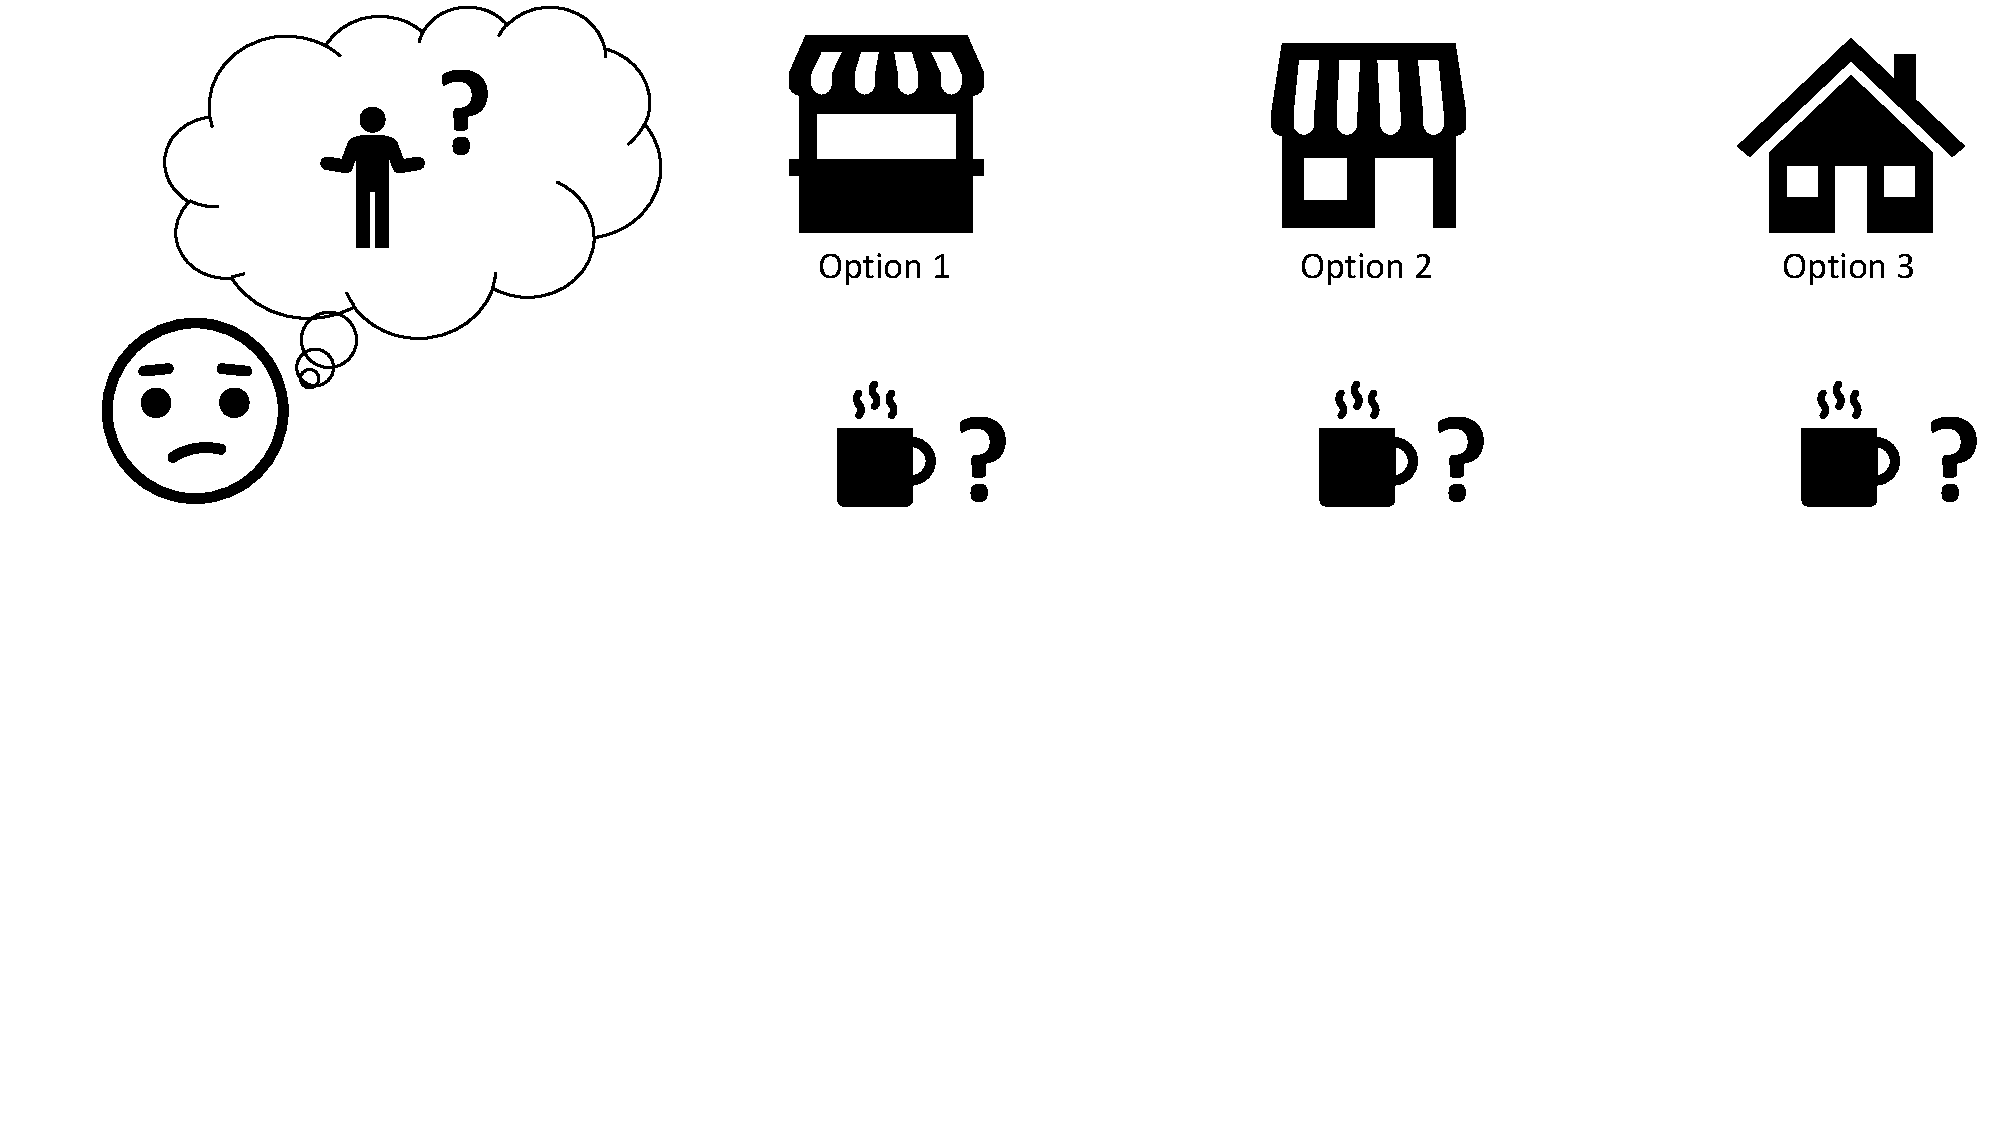
\includegraphics[width=1\textwidth]{Plots/CoffeExample.pdf}
    \vspace{-4cm}
    \caption[Coffe Shop Example]{How to choose a coffee shop. You are completely new in a city and you have multiple options, you do not know anything about the coffee from the different options.}
    \label{fig:Coffe_Example}
\end{figure}


%CW: 2nd paragraph introduces the explore-exploit dilemma. This is a crucial paragraph that needs to be clearly developed. I think the two alternatives are not laid out clearly. Perhaps look at the section in my thesis chapter for inspiration

The exploration--exploitation dilemma plays a crucial role in the reinforcement learning framework \citep{sutton2018reinforcement}, which provides computational solutions to problems where learning occurs through interactions with an environment. Modern approaches of reinforcement learning, which are used in machine learning and artificial intelligence are based on psychological models of associative learning \citep{sutton2018reinforcement}, which in turn can be traced back to early works of trial and error learning in animals. 

%CW: 3rd paragraph describes the structure of the thesis. I think this is isn't sufficiently informative for a naïve reader to understand, since it includes technical terms such as "bandit". Also, can you really discuss the bandit problem before the exploration. One additional point, you use the term "motivation of the thesis" wheres I think it's more of the focus of the thesis or the main question you are trying to solve. 
To discover how the coffee problem and other instances of the dilemma can be solved, we will begin this thesis with a history of reinforcement learning, which includes models of associative learning, such as classical and operant conditioning.
These models will provide the basis for a computational approach to reinforcement learning with which we will turn from animal learning to human reinforcement learning. We will focus on one of the main experimental paradigms to study the exploration-exploitation dilemma in humans: the bandit problem. We will shortly consider optimal solutions, however, these optimal solutions are intractable for real-world problems, which means, they do not provide a good framework for how humans solve the problem. 
This is why we will discuss potential strategies that provide heuristic solutions to the exploration-exploitation dilemma. These will be use as candidate models of human behavior. Considering Marr's levels of analysis \citep{dawson1998understanding}, which includes the computational level, e.g. what is happening , the representational level, e.g. what process is used, and as the last level the implementational level, e.g. how this process is physically integrated, we can use the models a way to understand the representational level and understand how the behavior (e.g. the computational level) is working as a process. Thus, not only can we observe the representational level with the help of observing the behavior in experiments, we can also understand the processes guiding the behavior with the representational level by using computational models. 
%with links process level theories of human learning.
Last but not least, I present a brief description of the empirical framework used to study the exploration-exploitation dilemma and a introduction to the major theories that guide the trade-off between exploration and exploitation in humans. In the light of the current discussion, I will close this chapter with an explanation of the main goals and hypothesis of this thesis. 

%CW: Here is where you should give a very short synopsis of what to expect in the introduction/thesis. I've rewritten substantial parts of this paragraph
Chapter \ref{ch:explo} of this thesis provides an overview of the reinforcement learning framework and the computational models we use for modeling human decision--makers. This includes an intuitive but sufficiently technical background for understanding the model comparison and analyses presented in later chapters.
Chapter \ref{ch:experiment} presents the experimental design and behavioral results of an experiment which studied the influence of time constraints on human learning and choice behavior in a multi-armed bandit task. 
Chapter \ref{ch:results} presents analyses using computational models to predict both choices and reaction times, in order to develop an understanding of the cognitive processes used by human decision--makers to navigate the exploration--exploitation dilemma. Chapter \ref{ch:discussion} provides concluding remarks and a discussion of limitations and future directions. 

\section[A history of reinforcement learning]{A history of reinforcement learning\\ {\large It's raining cats and dogs}} 

Historically, studies involved cats and dogs, like classical conditioning \citep{pavlov1927conditional} or the law of effect \citep{thorndike1927law}, which can be seen as the roots of reinforcement learning. 
%This section provides an introduction to reinforcement learning and its history in early research on human and animal learning. The roots of reinforcement learning can be traced back to Thorndike's (\citeyear{thorndike1927law}) law of effect and Pavlov's (\citeyear{pavlov1927conditional}) theory of classical conditioning, which were based on observations of learning in cats and dogs. %CW: rearranged the order to talk about cats and dogs 
\citet{thorndike1927law} investigated the role of learning in cats, and drawing on his observations he formulated the law of effect.
The law of effect states that whenever an agent receives a positive feedback, it is more likely to try the same action again. In contrast to negative feedback, the agent is more likely to avoid this action in the future.
These dynamics are the basis for learning through interactions with an environment (reinforcement learning).% Remember the coffee shop example: When you explore your environment and thus try a new coffee shop you will get a feedback which will influence your decision. It seems plausible that the law of effects applied to this scenario implies that if we received a good coffee, we are more likely to go to the exact same coffee shop again.
For the formulation of other important theories of learning not only cats but also dogs played a crucial role, as for example in classical conditioning \citep{pavlov1927conditional}. 
The main concept of classical conditioning is that you can learn that an event (or stimulus) can precede another event, so you can be more prepared when that event actually happens. However, in this thesis we are even more interested in the computational models that emerged in order to describe classical conditioning. One of these is the Rescorla Wagner Model \citep{rescorla1972theory}. This model paved the way from passive associations to active learning based on a prediction error.

\subsection{Classical Conditioning}
Ivan Pavlov accidentally discovered the learning concept of classical conditioning in 1927. Initially, he wanted to study the digestive system of dogs, but unintentionally, he observed that his dogs started to salivate when the caretaker arrived to give them food. Even before food was presented to the dogs, they started to respond in anticipation. This launched a series of experiments that would become the foundation for Pavlov's theory of classical conditioning \citep{pavlov1927conditional}.  

%\subsubsection{Pavlov's Dogs}
%CW: Terminology overload. CS, CR, US, UR,... Maybe acronyms help, maybe they don't.
In order to test his previous observation, Pavlov created an experiment where he introduced the sound of a metronome before the dogs received their food. After a few repetitions, the dogs began to show the same reaction as in his earlier observation with the caretaker: they began to salivate in anticipation of the food.
Pavlov called this response a \emph{conditioned response}. A conditioned response is learned when an \emph{unconditioned stimulus (US)} (e.g. food) is paired with a neutral stimulus (the sound). Usually the neutral stimulus is presented before the US. After several repetitions of pairing these stimuli, the neutral stimuli becomes the \emph{conditioned stimuli (CS)}. The sound becomes associated with the food. After learning that the sound precedes the food, the dogs already start to salivate when hearing the sound, because they learned that after hearing this sound food will be presented.
\begin{figure}
    \centering
    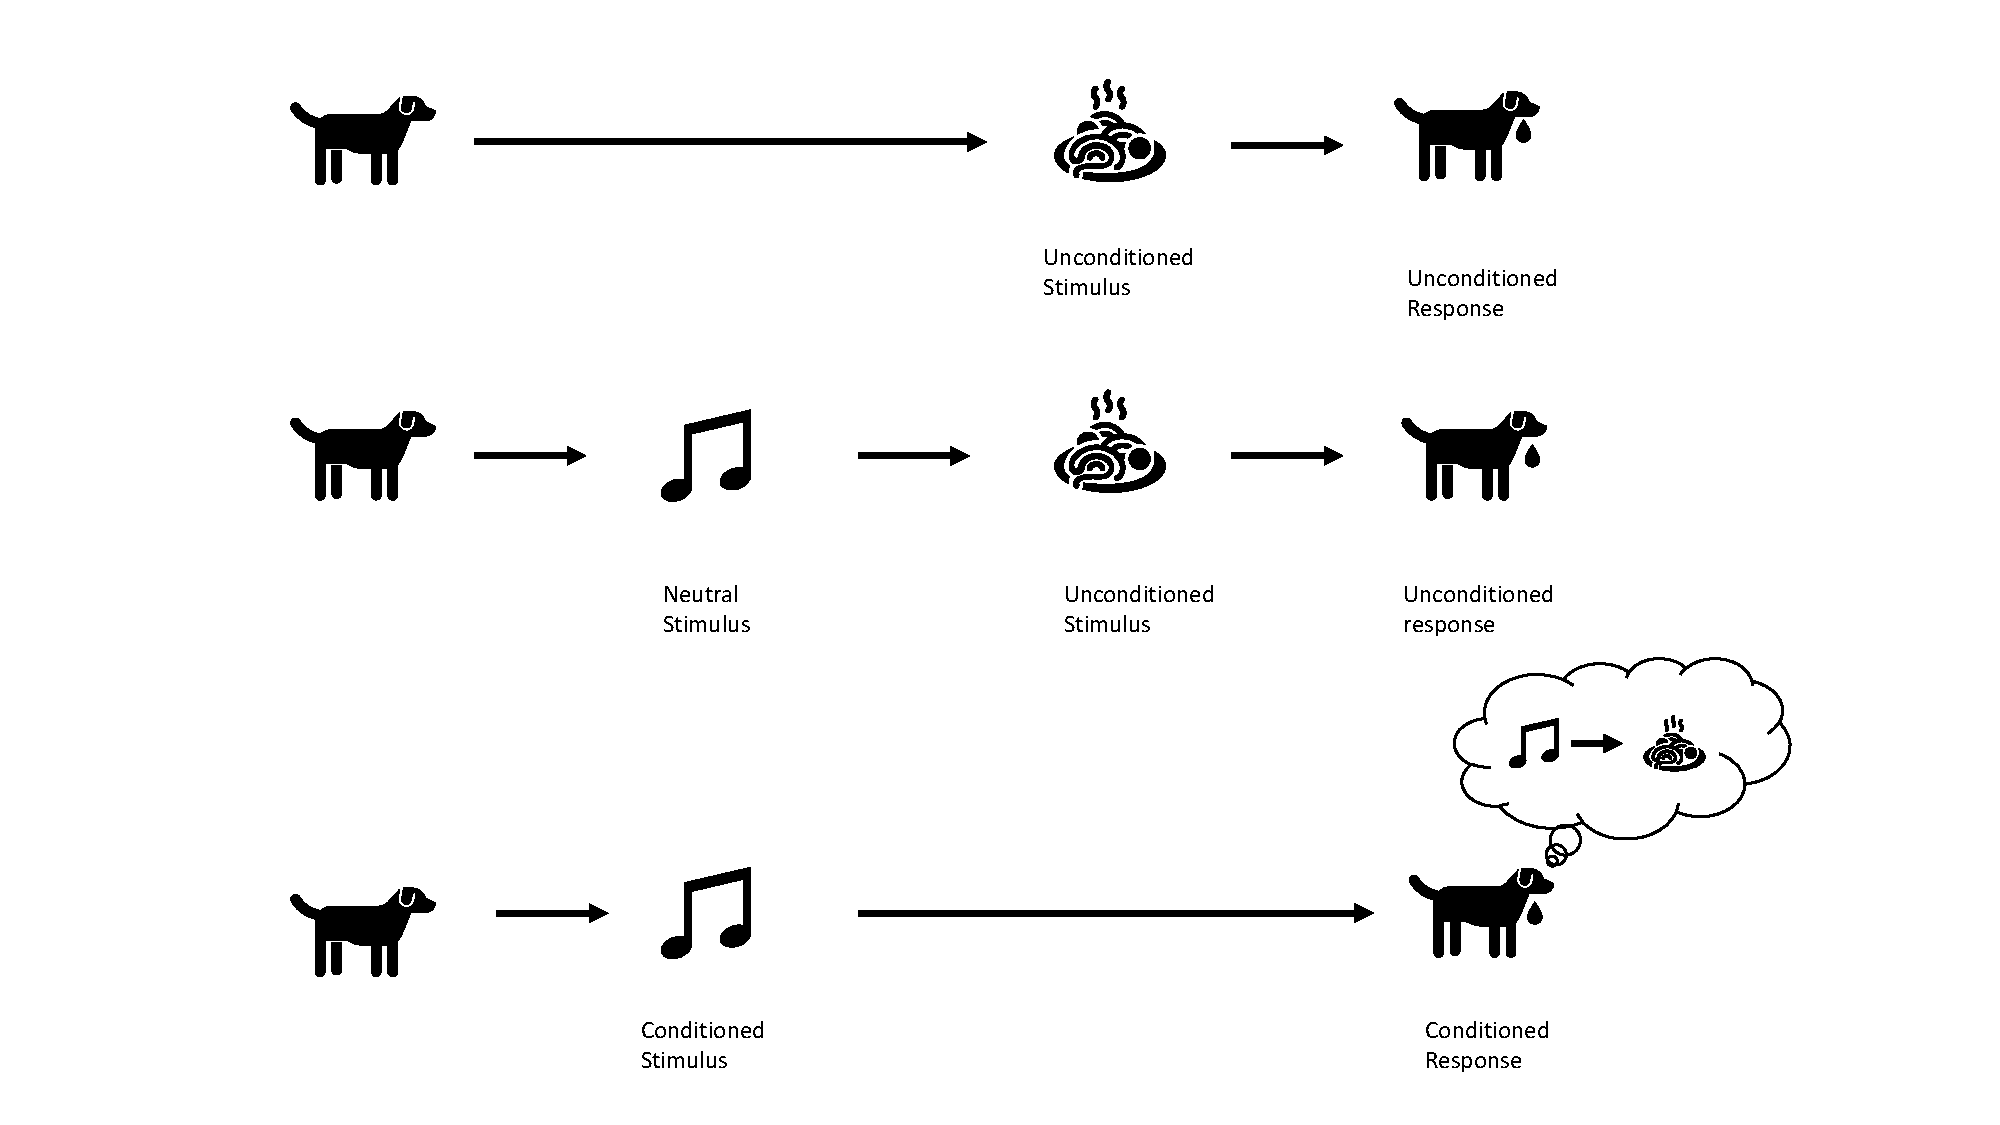
\includegraphics[width=1\textwidth]{Plots/ClassicalConditioning.pdf}
    \caption{Classical Conditioning}
    \label{fig:Classical_Conditioning}
\end{figure}

%To clarify this, let us consider the dogs once more. The arrival of the food is the unconditioned stimulus. In order to eat it, they produce saliva, which is the unconditioned response. A conditioned stimulus is introduced before the arrival of the food, which is the sound of the metronome. After a few trials, the dogs learn that the sound anticipates the arriving of the food. Thus, the dogs can already prepare to act when the food arrives. So they already start to produce saliva when they hear the sound of the metronome. 

What have we learned from Pavlov's experiments and what does it have to do with human learning? Through the concept of classical conditioning, we see that it is possible to learn to predict certain events. The dogs learned that the arrival of the caretaker or the sound of the metronome preceded the arrival of food. This is one of the essential features of reinforcement learning: trying to predict future outcomes.

\subsection{Trial and Error Learning}
Unlike classical conditioning trial and error learning is not focused on the learning to predict the future based on stimuli, it is more concerned with the behavior and the consequences of it, learning from actions. You associate specific actions with their outcome. This is the second main feature of reinforcement learning: association. 
Remember our coffee shop example: You are in a new environment with lots of different coffee shops to choose from and therefore with lots of possible actions. 
In order to choose actions which will lead to good outcomes, you need to try actions, which will most likely include errors.
There is the possibility to try a new option and thus taking an action from which you learn more about your environment but also about your future decisions. 

%\subsubsection{Law of Effect}
Thorndike introduced the Law of Effect \citep{thorndike1927law}, which says that actions that are followed by a satisfaction, will occur again in the same situations, whereas other actions taken in the same situation that are not followed by a positive effect are not. He also discovered that the stronger the satisfaction, the greater the action is associated with this kind of situation. Consequently, we see that the law of effect and reinforcement learning have the same essential principle: learning through interacting with the environment.

Thorndike studied this phenomenon using puzzleboxes \citep[pp.8-30]{thorndike1898animal}, which were a series locked boxes that could be opened by pulling various levers or buttons. In front of the box food was displayed, so that the cats inside were able to see the food. Cats were put into the box with no obvious way out. They had to find out which actions they had to perform in order to escape. They needed to pull or push specific button to get out.
The first time in the box, the cats scratched and tried many unsuccessful actions in order to escape. Eventually, the cats would happen upon the button or lever that would open the box and managed to escaped. During subsequent trials, the cat had already learned which actions helped it to escape the box.
%Therefore, reducing unsuccessful actions and promoting satisfying actions, which is called an associative linkage. %CW: Sentence fragment
The cats linked successful actions to the situations and upon encountering the situation again, these associated actions were chosen again to achieve the best reward they could get, namely escaping the box. 


\subsubsection{Behaviorism}
\cite{skinner1963operant} introduced operant conditioning, the idea of reinforcing behavior through rewards or punishment. Unlike classical conditioning, it focuses on the action and not on the stimuli that is presented. In order to examine his theory he created the Skinner box, a variation of Thorndike's puzzlebox. The box varies in the way that the main goal is not to escape but to pull a lever in order to gain food. This allowed him to observe animals over a longer period of time and he could thanks to his observations indeed conclude that the rats that were put into this box learned favourable behavior through interacting with the environment. This changed their behavior within the box entirely.   
He continued to examine this phenomenon with various experiments and found that this gave the possibility to shape the behavior of animals in specific directions. For example in a pigeon experiment, he was able to teach a pigeon to bowl a wooden ball. He did this by reinforcing specific behavior that in the end led to the pigeon learning to pick the wooden ball and throw it in the right direction. Unlike Thorndike, Skinner concluded that the right actions are learned over the accumulation of random actions that will lead to the correct action. 

\subsection{From Classical Conditioning to Prediction Error Learning}
%CW: Revisit my suggestion of passive vs. active learning
In 1972, \citeauthor{rescorla1972theory} created a mathematical model to account for blocking in classical conditioning\footnote{The Rescorla-Wagner model was not the first model to use a prediction error learning rule, but it is the most famous one. The first model was created by Bush and Mosteller\cite{bush1951mathematical},\cite{bush1951model} }\citep{rescorla1972theory}. The model is based on the assumption that the learning agent is faced with an unpredicted situation, e.g. when the predicted outcome is not the actual outcome.
The focus is on the relationship between a conditioned stimulus and an unconditioned stimulus. 
The learning of the CS is represented by the aggregate associative strength\footnote{A CS can consist of multiple component stimuli, each with an own associative strength, the combination of all those associative strength is the aggregated associative strength}, which adjust after each trial due to a predictive error. The aggregated associative strength says how reliable the CS predicts the US.
The prediction error is calculated by taking the difference between the asymptotic level of associative strength (or in easy: the point at which the US perfectly predicted) and the associative strength. If the prediction error is positive, the US can be learned and the associative strength is increasing after each trial until it is equal to the asymptotic level. Thus, if a new component stimuli is introduced, there is little to no learning effect, because the prediction error is already around zero. That is how the model accounts for blocking.

This is a new approach to learning in the sense that it is a more active kind of learning. The idea of calculating a prediction error includes actually predicting the future outcomes, whereas in classical condition, the process of learning is merely a passive association of stimuli and reward. Thus the idea of how we learn changed from passively learning associations to predict the outcome, check that prediction against the true outcome and update the belief to reduce the error in predicting the reward. 
From the idea of only associating rewards with specific actions the idea of how trial and error learning is accomplished changed to the idea of predicting the future, observing the presence and updating ones own beliefs in order to minimize the difference between what one calculated and what actually happened in order to predict more accurately the next time and thus improve future performance. 

This concept is similar to the delta-rule \citep{widrow1960adaptive}, a learning rule used in machine learning algorithms. It is also called the least mean square method, because it looks for the weights that will minimize the square of all errors.


\subsection{A Computational Approach to Reinforcement Learning}
In the history of the reinforcement learning two subsets emerged, one dealing with animal learning and the other one with dynamical programming. Dynamical programming \citep{bellman1960dynamic} was developed by Robert Bellermann in the 1950s and is concerned with optimal control \citep{sutton2018reinforcement}. 
Stochastic optimal control problems, and its solutions like Markov decision processes, are the problems that resemble the problems we considered the most. Markov decision processes is a formalization of sequential decision making \citep{sutton2018reinforcement}. This means they can be used to describe problems we have considered before.  
However, since dynamical programming deals with optimal solution, this as well as Markov decision processes, are computationally expensive and take a long time to be solved. We will consider a specific example of optimal control in the following section. 

\section{Human Reinforcement Learning}
Let us turn back to our coffee shop example. Imagine there are many coffee shops available in your neighborhood. Your goal is to accumulate the best coffee experience as you can. This might include some bad coffees but also exploring more shops to get an even better coffee experience. 
You have multiple options where to choose from. You could either rely on your previous knowledge and get a coffee where you would know how it is, or you try something new, where you have no previous knowledge of how good it is. Sometimes, you might not even have some previous knowledge but still need to decide between multiple options. How is this done? How do you decide? 
\citeauthor{thompson1933likelihood} studied choice problems and introduced the experimental design of bandit problems in 1933 \citep{thompson1933likelihood}, which are named after the slot machines in casinos. Bandit problems were studied not only in the field of psychology but also in the field of artificial intelligence and machine learning. Each field of study influenced the other fields, creating an interdisciplinary topic.   

\subsection{Bandit Problem}
Bandit problems are types of reinforcement learning problems with the exploration- exploitation dilemma as its core problem. It is an evaluative feedback problem, which means that a response is given about how good the chosen action was. The name and the problem were inspired by slot machines in casinos, which are called one armed bandits. When you pull the lever of such a machine it will give you a reward, if you are unlucky, you won't get any. The bandit problem in reinforcement learning is similarly structured, only that you always get a reward when you choose a lever. The levers are the given options. The most common type of bandit problem is the two armed bandit, which has two options. For example, you can imagine this as two slot machines next to each other or if we look at our coffee shop problem: you have two shops to choose from.
There are multiple versions of this problem and are all summarized under the term multi-armed or \textit{K}-armed bandit, so you can basically have any number of options available. 
In a classical experiment which uses the bandit problem, you have a limited amount of decisions and your main goal is to achieve the highest possible accumulated reward. The rewards are drawn from underlying probability functions, which are called reward functions. This just means that you do not only get the same reward from each option but there can be a variability in the rewards for each option. To make it more intuitive, think about the coffee example: you do not get the same quality of your coffee every time you buy one in the same shop; the quality can vary.

So we can say that our coffee is an instance of a multi-armed bandit problem. But how can we solve it? 

%The name and problem itself was inspired by slot machines in casinos. Those machines produce unknown rewards if you pull their lever. In the bandit problem, each arm of a bandit is inspired by one of those slot machines. Thus, if there is more than one arm, you can imagine as if you would sit in front of more than one of those slot machines and now you are able to decide which lever to pull.
%In this problem, you are faced with choosing between different choices. After each choice, you get a numerical reward as a feedback. Usually, the amount of choices is limited and the main goal is to achieve the highest possible total reward. 
%The simplest version of the multi-armed bandit problem is the two-armed bandit. There only two choices are available. It is commonly used in economics where one of the arm usually gives a steady reward while the other one produces more uncertain rewards, which are drawn from a probability distribution, or reward functions. There are of course, variations where both rewards are drawn from different reward functions.  
\paragraph{Gittins Index}
One way to find a solution to these problems can be achieved through dynamical programming, which is concerned with optimal solution strategies.  \cite{gittins1979bandit} found an optimal solution algorithm for some problems of the multi-armed bandit, however it is not robust and cannot solve all of the variations of the problem.
\citeauthor{gittins1979bandit} defines a solution, the Gittins Index, for problems with a \textit{finite} number of arms, that have fixed probabilities, and an \textit{infinite} horizon. This means only when you have endless opportunities to pick an option and nothing changes for the options, then the Gittins Index can find an optimal solution. This is usually impossible to achieve in real life.
As \cite{cohen2007should} pointed out, real world environments change over time and so the fixed probabilities condition and the stable number of arms condition are both violated. 
So we can see in theory, there could be an optimal solution, this is just not feasible to use. Humans are capable of solving these problems fairly well in real life. Thus we can assume that humans use another way to solve the problem than optimal solutions. But which?   
%However, in a special case of a two armed bandit, which was tested on foraging strategies of birds, \cite{krebs1978test} found that those birds did indeed find a nearly optimal solution.
%Calculating the Gittins Index is simply calculating the expected total future reward for each option, from those you just need to choose the best option and have an optimal solution. 

\section{Exploration versus Exploitation dilemma}
\cite{kaelbling1996reinforcement} describes the exploration versus exploitation dilemma as one of the fundamentals of reinforcement learning, which sets itself apart from other fields of machine learning. The dilemma is concerned with finding the right trade-off between exploration, reducing uncertainty in a new environment (thus gaining information about the environment) and exploitation, choosing those options that will give the highest reward based on the current knowledge of the environment. Exploration is helpful in the long run, in order to find the action that will give the best reward. Exploitation is helpful in gaining the currently known best rewards. Accordingly, the bandit problem is an instance of the exploration-exploitation dilemma and thus also our coffee shop example. 

As proposed by \cite{cohen2007should} the trade-off is not only about one specific problem, but rather includes a spectrum of problems, backed up by \cite{mehlhorn2015unpacking}, they propose that there is not only one concept explaining it, but rather various. Examples\footnote{\cite{hills2015exploration} offers a broad overview of areas which are concerned with the trade-off} of the exploration exploitation dilemma are: animal foraging \citep{cook2013exploration}, visual search \citep{chun1996just}, or risk tasks \citep{gonzalez2011instance}.

Furthermore, \cite{cohen2007should} identified various factors that influence the decision on problems in this area, for example: the familiarity of the environment or how stationary the environment stays.

One possibility to look at this trade-off is by considering strategies how to explore an environment. In which ways can you look at the different coffee shops and reduce your uncertainty about the quality of the coffee? 
\subsection{Exploration Strategies}
Full information models, like the Gittins Index are computational very expensive and cannot even perform under all circumstances. Another approach to solve or explore the environments are heuristics, which do not take all information into account \citep{parpart2018heuristics}, but perform reasonable well and even outperform optimal solution strategies \citep{gigerenzer1996reasoning, gigerenzer1999simple, katsikopoulos2010robust}. As \cite{gigerenzer2009homo} pointed out heuristics are solutions that perform well enough to a certain aspiration level. This means that there is a specific threshold to reach before accepting the solution. As we have seen with the Gittins Index, optimal solution strategies are bound to very specific problems and usually need full information about the environment, these information also need to be stable, e.g. they are not allowed to change over time. Therefore, we can assume that most real-world problems are intractable for those kinds of algorithms. Heuristics which do not take all information into account are another approach to solve these problems. Two kinds of heuristics that solve the exploration-exploitation dilemma are widely discussed: random exploration and directed exploration.

\paragraph{Random Exploration}
\begin{figure}
    \centering
    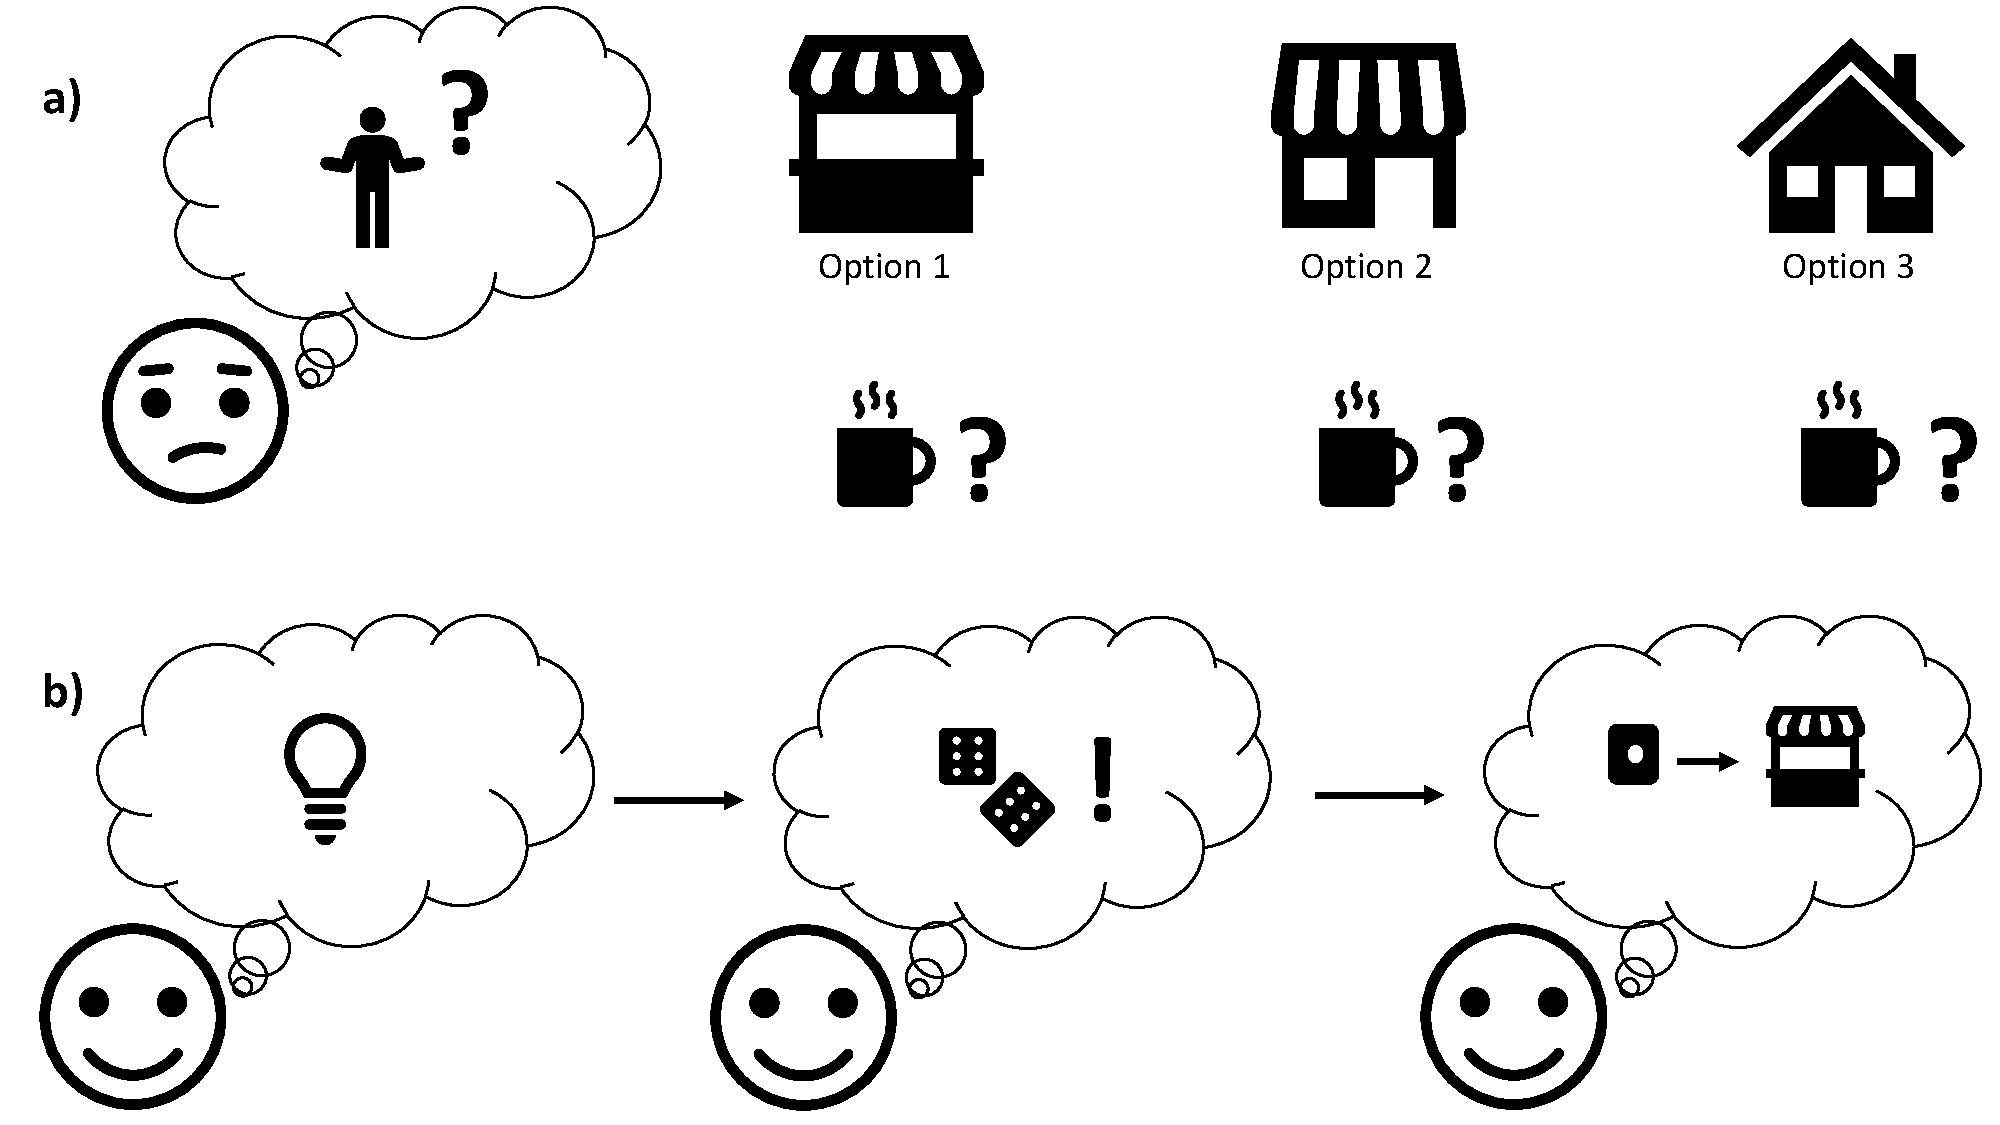
\includegraphics[width=1\textwidth]{Plots/RandomExploration.pdf}
    \caption[Random Exploration]{Random Exploration. In purely random exploration strategies each option has the same probability to be chosen, e.g. an option can be drawn by throwing a dice. If we consider Thompson Sampling, the dice is weighted for the option that has the best outcome, e.g. to always get a six in a dice.}
    \label{fig:RandomExploration}
\end{figure}

Random exploration is tightly associated with $\epsilon$-greedy algorithms. \cite{wilson2014humans} suggest that they reflect simple heuristics and have less computational cost than directed exploration strategies.  
$\epsilon$-greedy strategies are those kinds of strategies that nearly always preform greedily with only a small probability, $\epsilon$, of sampling randomly \citep[pp.27-28]{sutton2018reinforcement}. A greedy action would always choose the immediate best reward, thus ignoring exploration. In order to at least explore a bit, the probability of random selection is included. 

Thompson sampling is the best example of a random exploration strategy: It is a simple heuristic that performs reasonably well.
It was introduced by \cite{thompson1933likelihood} as a heuristic to solve a bandit problem.
Thompson sampling is random oriented, which means it randomly draws a value function from the posterior, which is our knowledge about the bandit e.g. the arms and what rewards can be expected. From this random draw it greedily chooses an action, maximizing the immediate reward. In easier terms: we have no complete knowledge of the process of the machine (the bandit), so we randomly assign parameters to it, draw a value function, from which we want to choose an action that will maximize the immediate outcome.

Random exploration is not as well researched as directed exploration, it is however, studied via model fitting.  
For example, \cite{daw2006cortical} studied a \textit{4}-armed bandit by comparing three different models. One of their models was a random exploration model, the $\epsilon$-greedy model, the other was a weighted belief update model, which uses the soft-max rule\footnote{options are weighted due to their estimated values}. Their last model was an extended version of their second model with an exploration bonus attached (a directed exploration model). \citeauthor{daw2006cortical} found that the third model with the exploration bonus did not have any evidence from the experimental data. Comparing the remaining two models, the soft-max model had the best fit. 

\paragraph{Directed Exploration}
\begin{figure}
    \centering
    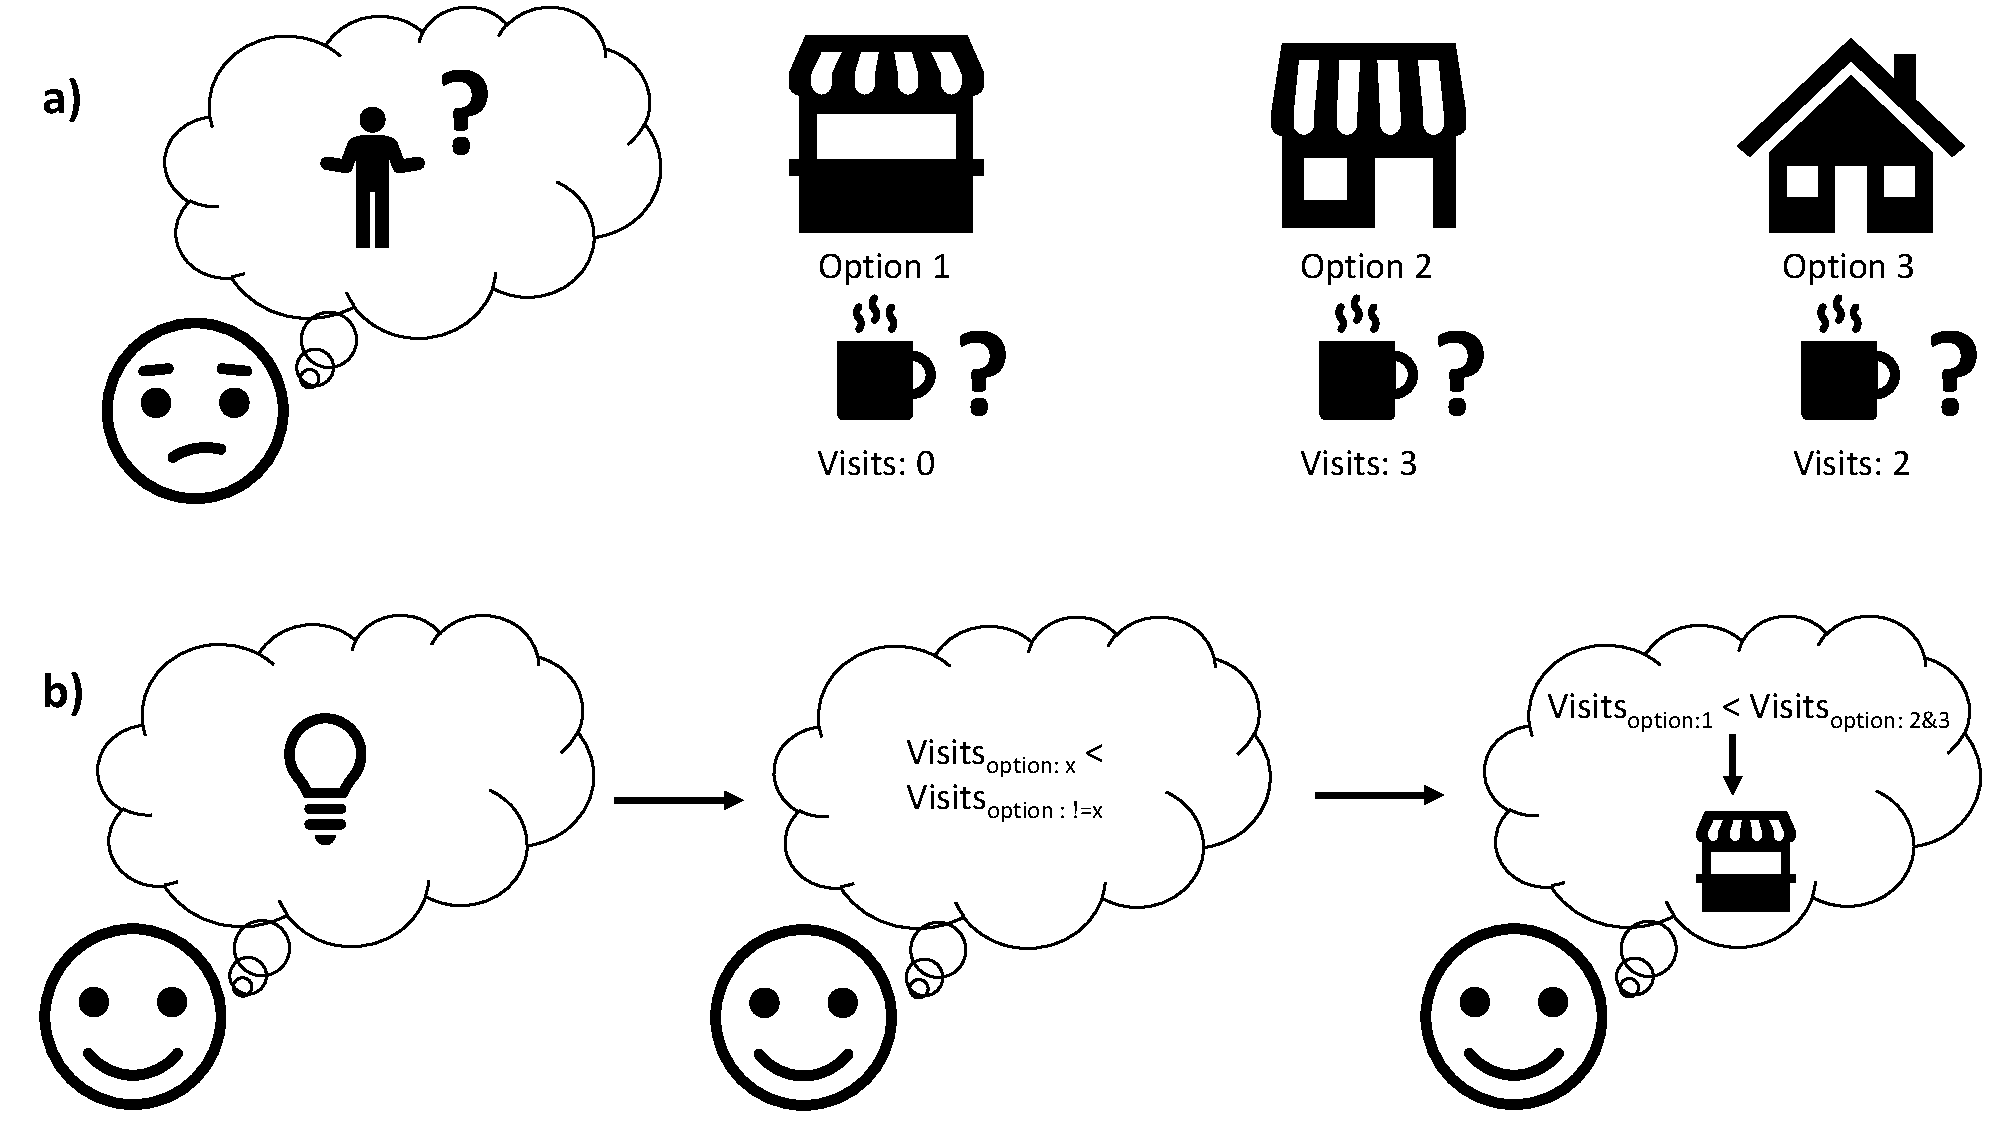
\includegraphics[width=1\textwidth]{Plots/DirectedExploration.pdf}
    \caption[Directed Exploration.]{Directed Exploration. In directed exploration strategies option which we know less about are more likely to be chosen, in order to gain more information andthus reduce uncertainty about the environment.}
    \label{fig:DirectedExploration}
\end{figure}
Directed exploration strategies like the Upper Confidence Bound (UCB) are derived from optimal decision making strategies \citep{wilson2014humans}. An exploration bonus is the main component of directed exploration behavior. The bonus leads to weighted exploration, this means that new options are not randomly selected but are encouraged by probabilities concerning their uncertainty. There has been evidence against the use of exploration bonuses in humans \citep{daw2006cortical}. However, more recently there has been more evidence found for the use of this strategy \citep{wilson2014humans, gershman2018deconstructing,knox2012nature, steyvers2009bayesian}.    
\cite{wilson2014humans} assume that there are two main reasons why some studies did not find any exploration bonus. Firstly, direct exploration might be difficult to identify due to a confound between information and reward. They assume that the gained information is confounded with the reward the option yielded, which makes it difficult to identify directed exploration. 
Secondly, they assume that there is an information- ambiguity interaction. In other words: the more information you have about an option, the more it is ambiguous. This would mean, that participants that avoid ambiguity avoid information seeking and prefer exploiting their current knowledge.


Unlike the Thompson sampling, the UCB \citep{auer2002finite} does not use immediate probabilities to decide which action to use, rather it works in the way that it uses an uncertainty bonus \citep{srinivas2009gaussian}. This basically means that more uncertain options (those you know less about) get a bonus, thus their probability of being picked is higher. This corresponds to the idea, that you accumulate the most information in order to exploit these information later.

\subsection{Current Theories}
The exploration versus exploitation dilemma can be described with examples of choice problems, e.g. finding a new favourite coffee shop in a town you recently moved to and in a more scientific way with the bandit problem. How to solve these problems is not well understood. Optimal solutions have constraints that are nearly impossible to obtain. There are currently two main strategies upon which humans solve these problems, random and directed exploration.  

The first option is exploring an environment only by chance, which is called random exploration. Thompson sampling is an example of random exploration.
The second option is directed exploration, where sampling from more uncertain option is encouraged by adding an uncertainty bonus. The UCB is an instance of this exploration strategy.

\cite{wilson2014humans} investigated the effect of the horizon on those two strategies in order to understand how humans use these strategies or if they use them at all. Their carefully designed experiment allowed to distinguish between both kinds of strategies, due to the assumption that a varying horizon influences the way of information seeking and can even produce decision noise. Therefore, they were able to conclude that both strategies are indeed used and vary depending on the horizon. Given the opportunity to explore more e.g. having a higher horizon, participants rather used a directed exploration strategy, while under a smaller horizon random exploration was used.
In alignment to this finding \cite{gershman2018deconstructing} proposed that humans use a mixture of both exploration strategies, thus promoting a hybrid model of the UCB and Thompson sampling. He concluded that under relative uncertainty\footnote{the relative uncertainty between the option} there was a faster response time, which is consistent with the UCB. Furthermore, under absolute uncertainty\footnote{the overall uncertainty} there was a slower response time, which indicated the Thompson sampling \cite{gershman2018uncertainty}.

\cite{zajkowski2017causal} found a distinction in brain activity for both exploration strategies. In their trans magnetic stimulation experiment, using the same paradigm as \cite{wilson2014humans} found that when inhibiting the right frontopolar cortex, there was a negative influence on the use of directed exploration. It had, however, no effect on random exploration.

If we consider Marr's three level hypothesis \citep{marr1976understanding}, we can argue that the exploration strategies would fall into the first level: The computational level, which is supposed to tell us what a system is doing, in our case, which action is chosen. The next step would be to take a look at the second level: The process level. This deals with how one actually ends up making a decision and how the processes behind it work. In other words: How are the decisions made and which processes are guiding this decision? 

\cite{gottlieb2018towards} suggest that learning is governed by curiosity. They assume that animals and humans have intrinsic motivations that value specific types of information gain more than others, which are independent of gaining rewards. This kind of behavior can be studied under active sampling tasks, which are variations of the bandit problem. In order to actually see this phenomenon it is important that the agents is allowed to freely choose which stimuli (or button or source of information) it wants to explore\footnote{in plain information gain tasks, the same behavior can also be seen, suggesting there is an intrinsic motivation to gain information}, before it has to chose an action. 
Considering signal detection theory, or evidence accumulation theories\footnote{the agent has uncertainty about states in the environment and has some control over how much information it sample to reduce this uncertainty} like the drift diffusion model, \cite{gottlieb2018towards} notes that these theories assume that the agent has some knowledge about how to identify relevant cues, without taking into consideration how the agents determines which cue is relevant. 
Furthermore, curiosity is linked to memory \citep{gruber2014states, kang2009wick} and attention \citep{jepma2012neural}, which are important factors in learning.


\cite{collins2012much} studied the relation of working memory and reinforcement learning. By creating a task that allowed to separate working memory specific effects on learning, they were able to set up a new computational model, that was able to better estimate single reinforcement processes. This model is composed of two smaller models one model free reinforcement learning model, which represent slow and cumulative learning, and a second model which represent the working memory and is fast but with limited capacity. In a study in 2014, they were able to test their model on data gathered by schizophrenic patients \citep{collins2014working}, which are know to perform poorly in reinforcement learning tasks. Due to fitting the data to the model, they were able to discover that the impairment for reinforcement learning were governed by deficits in working memory that effects reinforcement learning. 


As we have seen in the passages above from experimental behavior, we can draw conclusion about the process level from Marr's level hypothesis, which is how is the process working. Thus the remaining question is, how and what process governs random and directed exploration. 

\section{Motivation and hypotheses}
Learning by interacting with the environment first started in animal learning research and developed into the field of reinforcement learning. From a more passive kind of learning, theories changed into more active ideas like the error prediction, first introduced in the Rescorla-Wagner model. 

Most reinforcement learning questions can be studied with the exploration-exploitation dilemma, which focuses on the trade-off between exploring (reducing uncertainty about the environment) and exploiting (gaining rewards). In particular, the multi-armed bandit experimental design is used to investigate this dilemma. Optimal decision strategies like the Gittins Index prove to be inapplicable in real world scenarios, because it requires an infinite horizon and a stationary environment, both are criterion that are not in line with the real world, as there is a constantly changing environment and there can not be an infinite horizon. However, heuristics can perform reasonable well and sometimes outperform optimal decision strategies. Heuristics can be used as exploration strategies in the bandit problem.
As we have seen, humans use two kinds of exploration strategies, random and directed exploration, in order to solve the exploration-exploitation dilemma tasks like the bandit problem. These two heuristics can be formalized in the Thompson sampling for random exploration and the Upper Confidence Bound (UCB) for directed exploration. Both strategies are governed by uncertainty, but in different ways. Thompson sampling is governed by relative uncertainty while the UCB is governed by absolute uncertainty.

In order to understand the process managing these decision strategies, and thus get more insight into a process level theory, we applied time pressure onto a four armed bandit task. Due to manipulating the decision time, we reduce computation time, which will reduce the ability to sample and accumulate less evidence. This will give us insight into the underlying process which manages random and directed exploration, whether people use a combination of both or switch between them. 

\newpage




%\end{document}